\documentclass[a4paper, 12pt]{article}

%%%%%%%%%%%%
% Packages %
%%%%%%%%%%%%

\usepackage[french, english]{babel}

\usepackage[noheader]{packages/sleek}
\usepackage{packages/sleek-title}
\usepackage{packages/sleek-listings}
\usepackage{packages/sleek-theorems}

\usepackage{diagbox}

%%%%%%%%%%%%%%
% Title-page %
%%%%%%%%%%%%%%

\logo{resources/pdf/logo-uliege.pdf}
\institute{University of Liège}
%\faculty{}
%\department{y}
\title{Assignment 1}
\subtitle{Optimal decision making for complex problems}
\author{%
Maxime \textsc{Meurisse} (s161278)\\%
François \textsc{Rozet} (s161024)%
}
%\supervisor{}
%\context{}
\date{Academic year 2020-2021}

%%%%%%%%%%%%%%%%
% Bibliography %
%%%%%%%%%%%%%%%%

\addbibresource{resources/bib/references.bib}

%%%%%%%%%%%%
% Document %
%%%%%%%%%%%%

\begin{document}
    \maketitle
    
    \section{Implementation of the Domain}
    
    Our rule-based policy is defined as a \emph{clockwise-lap stationary policy}, \ie{} the agent follows the domain border in a clockwise fashion when it is on a border and goes right everywhere else. Formally,
    \begin{equation}\label{eq:clockwise.policy}
        \mu(x, y) = \begin{cases}
            (1, 0) & \text{if } x < n - 1 \text{ and } y = m - 1 \\
            (0, -1) & \text{if } x = n - 1 \text{ and } y > 0 \\
            (-1, 0) & \text{if } x > 0 \text{ and } y = 0 \\
            (0, 1) & \text{else}
        \end{cases}
    \end{equation}
    where $(x, y) \in X$ is the state of the agent and $n \times m$ the size of the domain instance.
    
    In the deterministic domain, the action proposed by the policy is always applied. However, in the stochastic domain, it is applied only if the noise $w \leq 0.5$. Otherwise, the state is updated to $(x, y) = (0, 0)$.
    
    Because $w$ is draw randomly from $\mathcal{U}(0, 1)$, both events have the same probability (\num{0.5}). Hence, this mechanism is equivalent to choosing $w$ as $0$ or $1$, with an equal probability. Formally, $w \sim \mathcal{U}\{0, 1\}$. Furthermore, the deterministic domain can be seen as a specialization of the stochastic one where $w$ is always $0$ ($w \sim \mathcal{U}\{0\}$). These considerations allow to simplify the implementation of the domain components.
    
    The policy \eqref{eq:clockwise.policy} has been simulated in the two domains through a single trajectory of 11 steps ($x_0$ to $x_{11}$), starting at initial state $x_0 = (3, 0)$, which is illustrated in Listing \ref{lst:simulated.domains}.
    
    \begin{lstlisting}[style=defaultFrameTB, gobble=8, caption={Simulated trajectories by applying policy \eqref{eq:clockwise.policy} in both domains.}, label={lst:simulated.domains}]
        Deterministic domain
        --------------------
        ((3, 0), (-1, 0), 5.0, (2, 0))
        ((2, 0), (-1, 0), 6.0, (1, 0))
        ((1, 0), (-1, 0), -3.0, (0, 0))
        ((0, 0), (0, 1), 1.0, (0, 1))
        ((0, 1), (0, 1), -5.0, (0, 2))
        ((0, 2), (0, 1), 0.0, (0, 3))
        ((0, 3), (0, 1), 19.0, (0, 4))
        ((0, 4), (1, 0), 10.0, (1, 4))
        ((1, 4), (1, 0), -8.0, (2, 4))
        ((2, 4), (1, 0), -5.0, (3, 4))
        ((3, 4), (1, 0), 9.0, (4, 4))
        
        Stochastic domain
        -----------------
        ((3, 0), (-1, 0), 5.0, (2, 0))
        ((2, 0), (-1, 0), 6.0, (1, 0))
        ((1, 0), (-1, 0), -3.0, (0, 0))
        ((0, 0), (0, 1), 1.0, (0, 1))
        ((0, 1), (0, 1), -5.0, (0, 2))
        ((0, 2), (0, 1), -3.0, (0, 0))
        ((0, 0), (0, 1), 1.0, (0, 1))
        ((0, 1), (0, 1), -5.0, (0, 2))
        ((0, 2), (0, 1), -3.0, (0, 0))
        ((0, 0), (0, 1), -3.0, (0, 0))
        ((0, 0), (0, 1), 1.0, (0, 1))
    \end{lstlisting}
    
    \section{Expected Return of a Policy}
    
    From the theory \cite{ernstinfo8003}, we know that
    \begin{equation}
        \norm{J^\mu - J^\mu_N}_\infty \leq \frac{\gamma^{N}}{1 - \gamma} B_{r}
    \end{equation}
    where $B_r = \norm{r}_\infty$ and $\gamma \in [0; 1)$ is the discount factor.
    It shows that we can estimate, up to a certain precision, $J^{\mu}$ by the functions $J^{\mu}_N$, which are defined by the recurrence equation
    \begin{equation}\label{eq:j.formulae}
        J^{\mu}_N(x) = \underset{w \sim p_{w}(\cdot \mid x, u)}{E}\left[r(x, \mu(x), w) + \gamma J^{\mu}_{N-1}(f(x, \mu(x), w))\right], \quad \forall N \geq 1
    \end{equation}
    where $J^{\mu}_0(x) \equiv 0$. To implement $J^\mu_N$, we decided to follow the dynamic programming (DP) principles and built a routine (a function) that iteratively computes $J^\mu_{i + 1}$ (for all $x \in X$) based on the values of $J^\mu_i$. Also, since we know that $w \sim \mathcal{U}\{0, 1\}$ (or $\mathcal{U}\{0\}$), the expectations were computed by averaging over the possible values of $w$ (either $0$ or $1$).
    
    For the choice of $N$, we decided to bound the infinite norm of the difference between $J^{\mu}$ and $J^{\mu}_N$ by the threshold $\epsilon = \num{e-3}$ since this value is numerically insignificant with respect to the rewards. Hence, we have to find $N$ such that
    \begin{align}
        \frac{\gamma^{N}}{1-\gamma} B_{r} & \leq \epsilon \nonumber \\
        \gamma^{N} & \leq \frac{\epsilon}{B_r}(1-\gamma) \nonumber \\
        N & \geq \log_{\gamma}\rbk{\frac{\epsilon}{B_r}(1-\gamma)} \label{eq:n.inequality}
    \end{align}
    The terms $\gamma$ and $B_r$ being fixed at \num{0.99} and \num{19}, respectively, we derive the smallest possible value of $N$, \ie{}
    \begin{equation}\label{eq:n.equality}
        N = \left\lceil \log_{\gamma}\rbk{\frac{\epsilon}{B_r}(1-\gamma)} \right\rceil = \num{1439} .
    \end{equation}
    
    For both domains, we computed $J^{\mu}_N(x, y)$ for the stationary policy \eqref{eq:clockwise.policy} at each state $(x, y) \in X$ (\cf{} Tables \ref{tab:j.values.deterministic} and \ref{tab:j.values.stochastic}).
    
    \begin{table}[H]
        \centering
        \begin{tabular}{c|c|c|c|c|c}
            \diagbox{$x$}{$y$} & $\bm{0}$ & $\bm{1}$ & $\bm{2}$ & $\bm{3}$ & $\bm{4}$ \\ \hline
            $\bm{0}$ & \num{-48.474} & \num{-49.974} & \num{-45.428} & \num{-45.887} & \num{-65.542} \\ \hline
            $\bm{1}$ & \num{-50.989} & \num{-47.328} & \num{-55.887} & \num{-65.542} & \num{-76.305} \\ \hline
            $\bm{2}$ & \num{-44.479} & \num{-69.797} & \num{-74.542} & \num{-76.305} & \num{-68.995} \\ \hline
            $\bm{3}$ & \num{-39.035} & \num{-44.812} & \num{-49.305} & \num{-68.995} & \num{-64.642} \\ \hline
            $\bm{4}$ & \num{-32.644} & \num{-52.318} & \num{-68.795} & \num{-72.107} & \num{-74.386} \\
        \end{tabular}
        \caption{$J^{\mu}_N(x, y)$ for all $(x, y) \in X$ in the deterministic domain; $N = 1439$.}
        \label{tab:j.values.deterministic}
    \end{table}

    \begin{table}[H]
        \centering
        \begin{tabular}{c|c|c|c|c|c}
            \diagbox{$x$}{$y$} & $\bm{0}$ & $\bm{1}$ & $\bm{2}$ & $\bm{3}$ & $\bm{4}$ \\ \hline
            $\bm{0}$ & \num{-121.103} & \num{-121.529} & \num{-116.330} & \num{-110.876} & \num{-119.052} \\ \hline
            $\bm{1}$ & \num{-122.892} & \num{-114.805} & \num{-115.876} & \num{-119.052} & \num{-126.476} \\ \hline
            $\bm{2}$ & \num{-119.277} & \num{-120.604} & \num{-123.552} & \num{-126.476} & \num{-123.294} \\ \hline
            $\bm{3}$ & \num{-117.988} & \num{-115.369} & \num{-112.976} & \num{-123.294} & \num{-119.895} \\ \hline
            $\bm{4}$ & \num{-116.850} & \num{-129.286} & \num{-133.943} & \num{-129.747} & \num{-127.171} \\
        \end{tabular}
        \caption{$J^{\mu}_N(x, y)$ for all $(x, y) \in X$ in the stochastic domain; $N = 1439$.}
        \label{tab:j.values.stochastic}
    \end{table}
    
    \section{Optimal Policy}
    
    The equivalent \emph{Markov Decision Process} (MDP) of the domain(s) can be obtained by computing the transition probability $p(x' \mid x, u)$ and the expected reward $r(x, u)$ using, respectively,
    \begin{align}
        p\left(x' \mid x, u\right) & = \underset{w \sim p_{w}(\cdot \mid x, u)}{E} \sbk{I_{\cbk{x' = f(x, u, w)}}} \quad \forall x, x' \in X, u \in U \\
        r(x, u) & = \underset{w \sim p_{w}(\cdot \mid x, u)}{E}[r(x, u, w)] \quad \forall x \in X, u \in U
    \end{align}
    where $I_{\cbk{logical}} = 1$ if $logical$ is true and $0$ else. Computing the transition probability and the expected reward is straight forward.
    
    Then, the state-action value functions $Q_N(x, u)$ are evaluated with the recurrence equation
    \begin{equation}\label{eq:q.function.recursive}
        Q_{N}(x, u) = r(x, u) + \gamma \sum_{x^{\prime} \in X} p(x' \mid x, u) \max_{u^{\prime} \in U} Q_{N-1}\left(x^{\prime}, u^{\prime}\right), \quad \forall N \geq 1
    \end{equation}
    with $Q_0(x, u) \equiv 0$. Similarly to $J^\mu_N$, we used to DP principles to implement a routine generating the sequence of $Q$-functions. Interestingly, equation \eqref{eq:q.function.recursive} can be expressed as basic matrix operations like element-wise sums and scalar products, which we took advantage of in order to make the routine efficient.
    
    Concerning $N$, we have to find $N$ such that $\mu^*_{N'} \equiv \mu^*_N$ for all $N' \geq N$ where
    \begin{equation}\label{eq:N-optimal.policy}
        \mu_{N}^{*}(x) \in \arg \max_{u \in U} Q_{N}(x, u) .
    \end{equation}
    At first sight, we could think that finding the smallest $N$ such that $\mu^*_{N+1} \equiv \mu^*_N$ is sufficient, but it is not. In fact, there is no way to guarantee that the inferred policy won't change latter on. There even could be an infinite periodic oscillation between different policies having the same return. However, we have the relation
    \begin{equation}
        \norm{J^{\mu^*} - J^{\mu^*_N}}_\infty \leq \frac{2 \gamma^{N}}{(1 - \gamma)^2} B_{r}
    \end{equation}
    to impose a bound on the difference of the returns from $\mu^*_N$ and $\mu^*$. With the same development (and parameters) as \eqref{eq:n.inequality}, we obtain
    \begin{equation}\label{eq:n.equation.q}
        N = \left\lceil \log_{\gamma} \rbk{\frac{\epsilon}{2 B_r}(1-\gamma)^2} \right\rceil = \num{1966} .
    \end{equation}
    
    The inferred policies $\mu^*_N$ for both domains are presented in Tables \ref{tab:optimal.policy.deterministic} and \ref{tab:optimal.policy.stochastic}.
    
    \begin{table}[H]
        \centering
        \begin{tabular}{c|c|c|c|c|c}
            \diagbox{$x$}{$y$} & $\bm{0}$ & $\bm{1}$ & $\bm{2}$ & $\bm{3}$ & $\bm{4}$ \\ \hline
            $\bm{0}$ & (1, 0) & (0, 1) & (0, 1) & (0, 1) & (-1, 0) \\ \hline
            $\bm{1}$ & (0, 1) & (0, 1) & (0, 1) & (0, 1) & (-1, 0) \\ \hline
            $\bm{2}$ & (-1, 0) & (0, 1) & (-1, 0) & (-1, 0) & (-1, 0) \\ \hline
            $\bm{3}$ & (-1, 0) & (0, 1) & (0, 1) & (-1, 0) & (-1, 0) \\ \hline
            $\bm{4}$ & (-1, 0) & (0, 1) & (-1, 0) & (-1, 0) & (0, -1) \\
        \end{tabular}
        \caption{$\mu^*_N(x, y)$ for all $(x, y) \in X$ in the deterministic domain; $N = 1966$.}
        \label{tab:optimal.policy.deterministic}
    \end{table}
    
    \begin{table}[H]
        \centering
        \begin{tabular}{c|c|c|c|c|c}
            \diagbox{$x$}{$y$} & $\bm{0}$ & $\bm{1}$ & $\bm{2}$ & $\bm{3}$ & $\bm{4}$ \\ \hline
            $\bm{0}$ & (1, 0) & (1, 0) & (1, 0) & (0, 1) & (-1, 0) \\ \hline
            $\bm{1}$ & (0, 1) & (0, 1) & (0, 1) & (0, 1) & (-1, 0) \\ \hline
            $\bm{2}$ & (-1, 0) & (0, 1) & (-1, 0) & (1, 0) & (-1, 0) \\ \hline
            $\bm{3}$ & (0, -1) & (0, 1) & (0, 1) & (0, -1) & (0, -1) \\ \hline
            $\bm{4}$ & (-1, 0) & (0, 1) & (-1, 0) & (-1, 0) & (1, 0) \\
        \end{tabular}
        \caption{$\mu^*_N(x, y)$ for all $(x, y) \in X$ in the stochastic domain; $N = 1966$.}
        \label{tab:optimal.policy.stochastic}
    \end{table}
    
    We also computed $J^{\mu^*_N}_N$ with the previously implemented routine (\cf{} Tables \ref{tab:j.optimal.values.deterministic} and \ref{tab:j.optimal.values.stochastic}).
    
    \begin{table}[H]
        \centering
        \begin{tabular}{c|c|c|c|c|c}
            \diagbox{$x$}{$y$} & $\bm{0}$ & $\bm{1}$ & $\bm{2}$ & $\bm{3}$ & $\bm{4}$ \\ \hline
            $\bm{0}$ & \num{1842.031} & \num{1857.19} & \num{1881} & \num{1900} & \num{1900} \\ \hline
            $\bm{1}$ & \num{1854.576} & \num{1870.279} & \num{1880.09} & \num{1891} & \num{1900} \\ \hline
            $\bm{2}$ & \num{1842.031} & \num{1855.576} & \num{1870.279} & \num{1881.09} & \num{1891} \\ \hline
            $\bm{3}$ & \num{1828.61} & \num{1848.01} & \num{1863.646} & \num{1863.279} & \num{1864.09} \\ \hline
            $\bm{4}$ & \num{1816.324} & \num{1826.52} & \num{1849.01} & \num{1863.646} & \num{1842.01} \\
        \end{tabular}
        \caption{$J^{\mu^*_N}_N(x, y)$ for all $(x, y) \in X$ in the deterministic domain; $N = 1966$.}
        \label{tab:j.optimal.values.deterministic}
    \end{table}
    
    \begin{table}[H]
        \centering
        \begin{tabular}{c|c|c|c|c|c}
            \diagbox{$x$}{$y$} & $\bm{0}$ & $\bm{1}$ & $\bm{2}$ & $\bm{3}$ & $\bm{4}$ \\ \hline
            $\bm{0}$ & \num{159.446} & \num{159.637} & \num{163.052} & \num{172.13} & \num{172.13} \\ \hline
            $\bm{1}$ & \num{159.637} & \num{163.052} & \num{164.903} & \num{167.63} & \num{172.13} \\ \hline
            $\bm{2}$ & \num{159.446} & \num{160.137} & \num{163.052} & \num{167.213} & \num{167.63} \\ \hline
            $\bm{3}$ & \num{159.259} & \num{162.196} & \num{167.313} & \num{162.196} & \num{167.213} \\ \hline
            $\bm{4}$ & \num{159.259} & \num{155.713} & \num{162.196} & \num{167.213} & \num{162.229} \\
        \end{tabular}
        \caption{$J^{\mu^*_N}_N(x, y)$ for all $(x, y) \in X$ in the stochastic domain; $N = 1966$.}
        \label{tab:j.optimal.values.stochastic}
    \end{table}
    
    \newpage
    
    \section{System Identification}

    From a given trajectory $h_t = (x_0, u_0, r_0, x_1, u_1, r_1, \dots, u_{t-1}, r_{t-1}, x_t)$, we can estimate $r(u, x)$ and $p(x' \mid x, u)$ by using, respectively,
    \begin{align}
        \hat{r}(x, u) & = \frac{1}{\abs{A_h(x, u)}} \sum_{i \in A_h(x, u)} r_i, \\
        \hat{p}(x' \mid x, u) & = \frac{1}{\abs{A_h(x, u)}} \sum_{i \in A_h(x, u)} I_{\cbk{x_{i+1} = x'}},
    \end{align}
    where $A_h(x, u)$ is the set of indices $\cbk{i \mid x_i = x, u_i = u}$. However, this procedure is computationally expensive. Instead, we implemented the algorithm described in the course (slide 29 of the first lecture) to update iteratively $\hat{r}$ and $\hat{p}$.
    
    However, this algorithm doesn't handle the case where a state-action pair $(x, u)$ isn't represented in the trajectory. In this case, we assumed that the transitions from $(x, u)$ to any state $x'$ were equally likely, \ie{}
    \begin{equation}
        p(x' \mid x, u) = \frac{1}{\abs{X}} = \frac{1}{n m} \quad \forall x' \in X.
    \end{equation}
    
    We applied the algorithm on a fixed trajectory $h_T$ of length $T = \num{e6}$, generated by a random uniform policy. To study the convergence of $\hat{r}$ and $\hat{p}$ towards $r$ and $p$, we computed them on truncated sections $h_t$ of $h_T$, with $t = 1, 100, 1000, \dots, \num{e6}$. The convergence of $\hat{p}$ and $\hat{r}$ towards $p$ and $r$, for both domains, are shown in Figures \ref{fig:si.convergence.speeds.deterministic} and \ref{fig:si.convergence.speeds.stochastic}.
    
    \begin{figure}[H]
        \centering
        \begin{subfigure}[b]{0.47\textwidth}
            \centering
            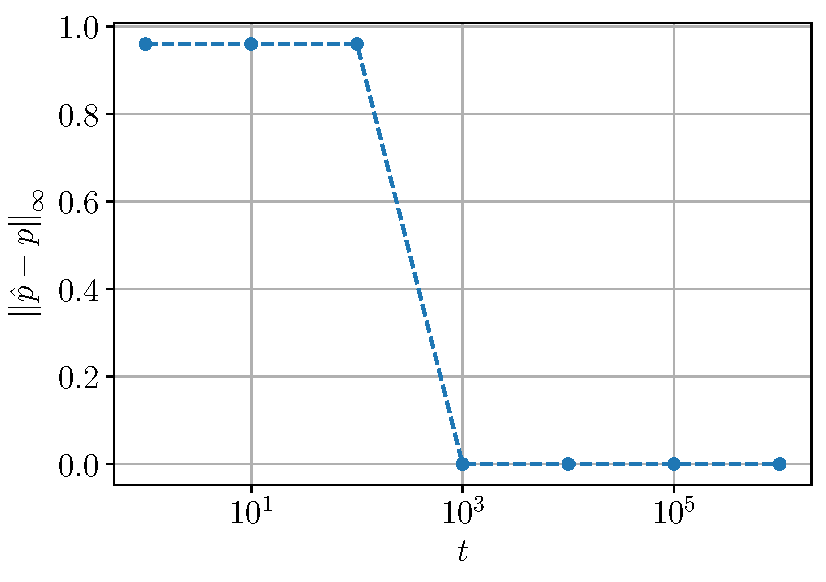
\includegraphics[width=\textwidth]{resources/pdf/4_p_deterministic.pdf}
        \end{subfigure}
        \hfill
        \begin{subfigure}[b]{0.47\textwidth}
            \centering
            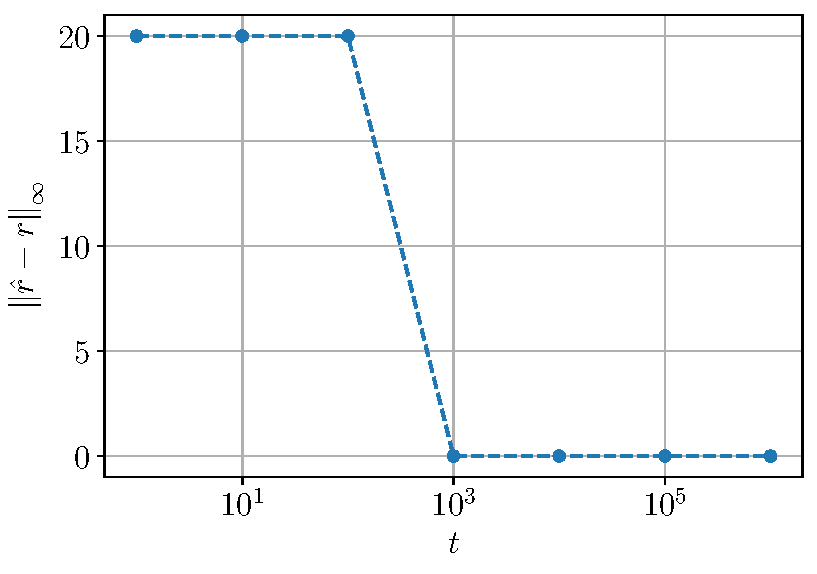
\includegraphics[width=\textwidth]{resources/pdf/4_r_deterministic.pdf}
        \end{subfigure}
        \caption{Convergence of $\hat{p}$ and $\hat{r}$ in the deterministic domain.}
        \label{fig:si.convergence.speeds.deterministic}
    \end{figure}
    
    In the deterministic domain, both $\hat{p}$ and $\hat{r}$ converged after $\num{e3}$ steps in the trajectory.
    
    \begin{figure}[h]
        \begin{subfigure}[b]{0.47\textwidth}
            \centering
            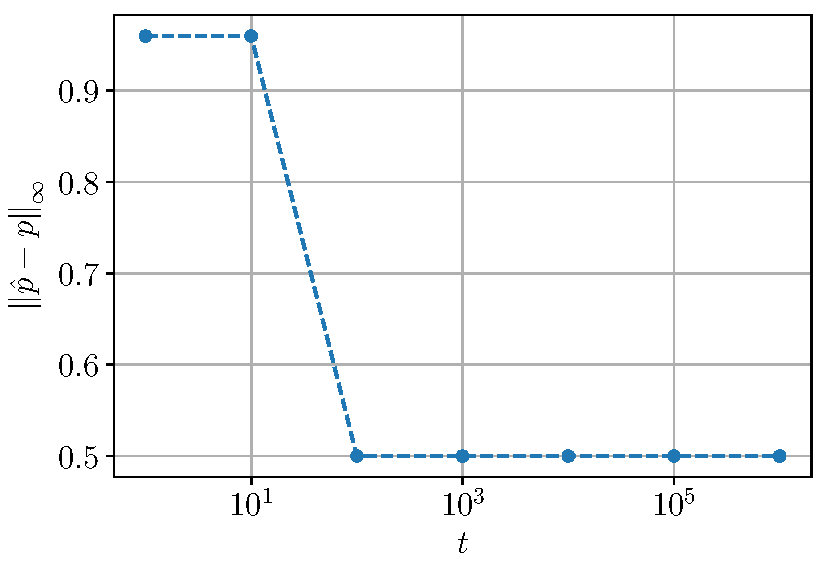
\includegraphics[width=\textwidth]{resources/pdf/4_p_stochastic.pdf}
        \end{subfigure}
        \hfill
        \begin{subfigure}[b]{0.47\textwidth}
            \centering
            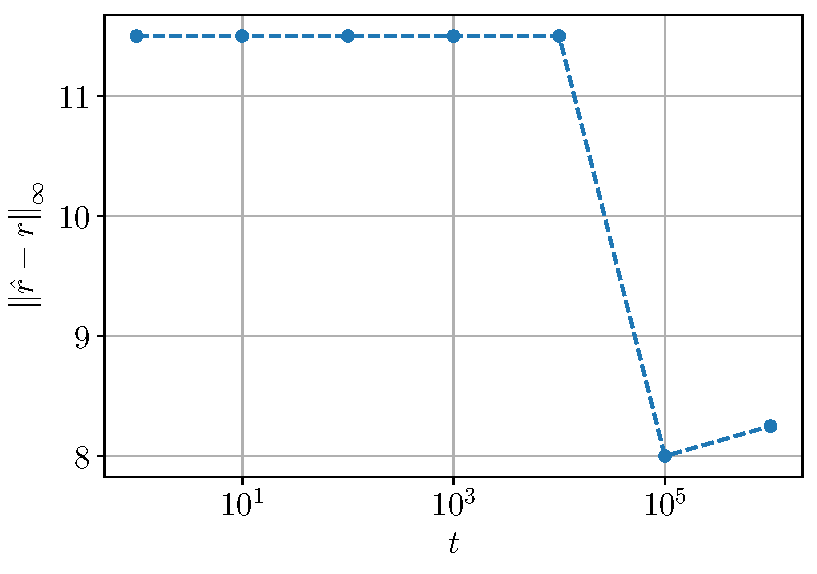
\includegraphics[width=\textwidth]{resources/pdf/4_r_stochastic.pdf}
        \end{subfigure}
        \caption{Convergence of $\hat{p}$ and $\hat{r}$ in the stochastic domain.}
        \label{fig:si.convergence.speeds.stochastic}
    \end{figure}
    
    In the stochastic domain, even after $\num{e6}$ steps, $\hat{p}$ and $\hat{r}$ have not yet fully converged. This behavior is easily explained. In order to have accurate estimates of $r$ and $p$, the trajectory needs to visit at least a few times every state-action pairs. Using the Markov chain theory, one can easily prove that, in the deterministic domain, a random uniform policy will have visited all pairs with high probability in the order of \num{e3} steps. But, in the stochastic case, there is a $0.5$ chance to be teleported to $(0, 0)$ at all time. Hence, the probability to reach the furthest states (\eg{} $(4, 4)$) is significantly lower. Using the same theory, it can be shown that it requires to the order of \num{e7} steps to have visited every pair with high probability, which would have required a lot of memory (assuming the trajectory is stored) and computations. Furthermore, increasing the number of visits, and therefore the trajectory length, will improve $\hat{r}$ and $\hat{p}$ as they are approximations of expectations. Although, in the deterministic domain, a single visit is enough. In our case, we settled for a trajectory length of \num{e6} as it is large enough to observe a bit of convergence in the stochastic domain.
    
    From estimates $\hat{r}$ and $\hat{p}$, we can compute the $\hat{Q}$-functions exactly like $Q$-functions by replacing $r$ and $p$ by respectively $\hat{r}$ and $\hat{p}$ in relation \eqref{eq:q.function.recursive}.
    
    Using the routine(s) implemented in previous sections, we computed $\hat{Q}_N$ with $N = \num{1966}$ from relation \eqref{eq:n.equation.q}. Once again, to study its convergence towards $Q_N$, we computed $\hat{Q}_N$ on the same truncated sections $h_t$ of $h_T$.
    
    The infinite norms between $\hat{Q}_N$ and $Q_N$ on both domains are shown in Figure \ref{fig:si.q.convergence.speeds}.
    
    \begin{figure}[h]
        \begin{subfigure}[b]{0.47\textwidth}
            \centering
            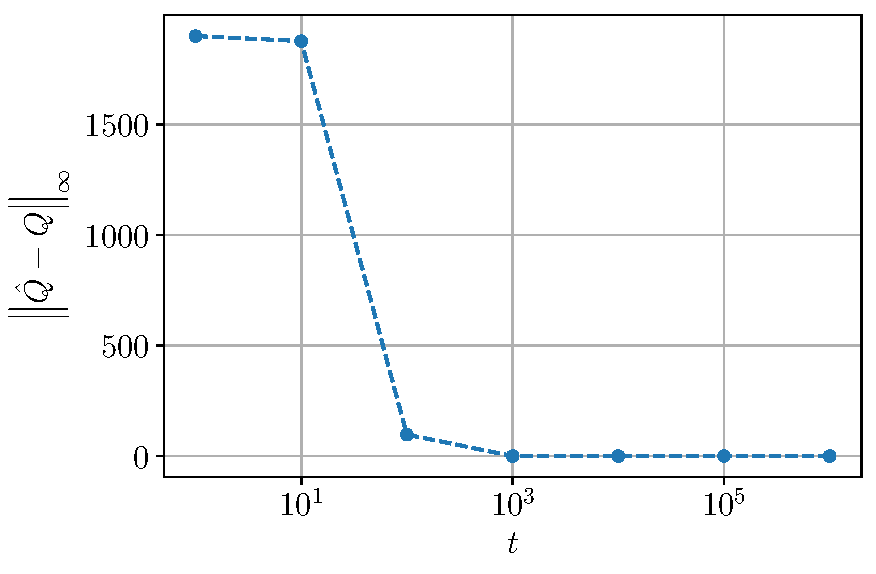
\includegraphics[width=\textwidth]{resources/pdf/4_Q_deterministic.pdf}
            \caption{Deterministic domain.}
        \end{subfigure}
        \hfill
        \begin{subfigure}[b]{0.47\textwidth}
            \centering
            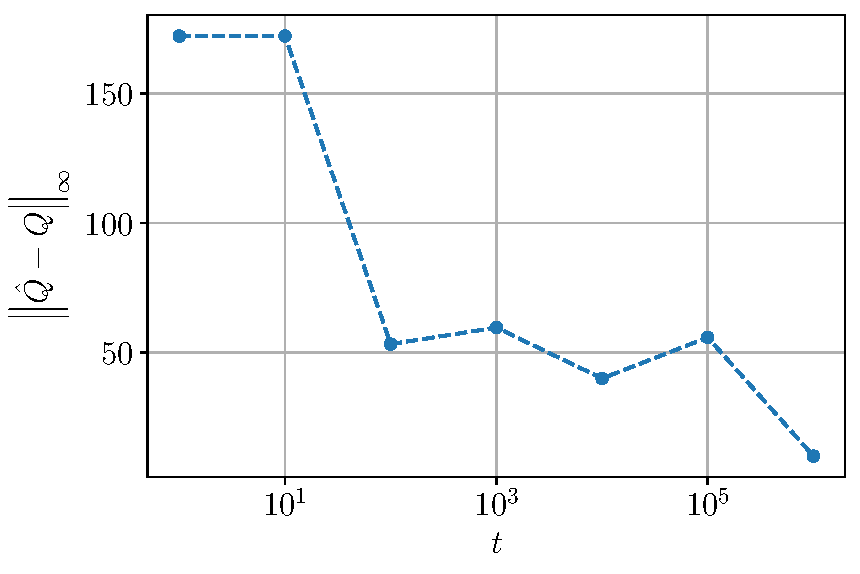
\includegraphics[width=\textwidth]{resources/pdf/4_Q_stochastic.pdf}
            \caption{Stochastic domain.}
        \end{subfigure}
        \caption{Convergence of $\hat{Q}_N$ towards $Q_N$.}
        \label{fig:si.q.convergence.speeds}
    \end{figure}
    
    Again, one can see that, in the deterministic domain, $\hat{Q}_N$ converged to $Q_N$ after $\num{e3}$ steps while in the stochastic case, it didn't even after $\num{e6}$ steps.

    An approximated optimal policy $\hat{\mu}^*_N$ can be directly derived by replacing $Q_N$ by $\hat{Q}_N$ in relation \eqref{eq:N-optimal.policy} and the best approximation is reached when $\hat{Q}_N$ has converged to $Q_N$. For the deterministic case, this length can be chosen as $\num{e3}$ but, for the sake of simplicity, we computed $\hat{Q}_N$ with the highest trajectory length (\num{e6}) for both domains.
    
    The obtained policies are shown in Tables \ref{tab:si.estimated.optimal.policy.deterministic} et \ref{tab:si.estimated.optimal.policy.stochastic}.
    
    \begin{table}[h]
        \centering
        \begin{tabular}{c|c|c|c|c|c}
            \diagbox{$x$}{$y$} & $\bm{0}$ & $\bm{1}$ & $\bm{2}$ & $\bm{3}$ & $\bm{4}$ \\ \hline
            $\bm{0}$ & (1, 0) & (0, 1) & (0, 1) & (0, 1) & (-1, 0) \\ \hline
            $\bm{1}$ & (0, 1) & (0, 1) & (0, 1) & (0, 1) & (-1, 0) \\ \hline
            $\bm{2}$ & (-1, 0) & (0, 1) & (-1, 0) & (-1, 0) & (-1, 0) \\ \hline
            $\bm{3}$ & (-1, 0) & (0, 1) & (0, 1) & (-1, 0) & (-1, 0) \\ \hline
            $\bm{4}$ & (-1, 0) & (0, 1) & (-1, 0) & (-1, 0) & (0, -1) \\
        \end{tabular}
        \caption{$\hat{\mu}^*_N(x, y)$ for all $(x, y) \in X$ in the deterministic domain; $N = 1966$.}
        \label{tab:si.estimated.optimal.policy.deterministic}
    \end{table}
    
    \begin{table}[H]
        \centering
        \begin{tabular}{c|c|c|c|c|c}
            \diagbox{$x$}{$y$} & $\bm{0}$ & $\bm{1}$ & $\bm{2}$ & $\bm{3}$ & $\bm{4}$ \\ \hline
            $\bm{0}$ & (1, 0) & (1, 0) & (1, 0) & (0, 1) & (0, 1) \\ \hline
            $\bm{1}$ & (0, 1) & (0, 1) & (0, 1) & (0, 1) & (-1, 0) \\ \hline
            $\bm{2}$ & (-1, 0) & (0, 1) & (1, 0) & (1, 0) & (-1, 0) \\ \hline
            $\bm{3}$ & (0, -1) & (0, 1) & (0, 1) & (-1, 0) & (1, 0) \\ \hline
            $\bm{4}$ & (-1, 0) & (0, 1) & (-1, 0) & (-1, 0) & (1, 0) \\
        \end{tabular}
        \caption{$\hat{\mu}^*_N(x, y)$ for all $(x, y) \in X$ in the stochastic domain; $N = 1966$.}
        \label{tab:si.estimated.optimal.policy.stochastic}
    \end{table}
    
    Using the routine inspired from \eqref{eq:j.formulae}, we get $J^{\mu^*_N}_N$ (\cf{} Tables \ref{tab:j.optimal.values.deterministic} and \ref{tab:j.optimal.values.stochastic}), previously computed, along with $J^{\hat{\mu}^*_N}_N$ (\cf{} Tables \ref{tab:si.estimated.j.optimal.values.deterministic} and \ref{tab:si.estimated.j.optimal.values.stochastic}) for each state $(x, y)$ in both domains.
    
    \begin{table}[H]
        \centering
        \begin{tabular}{c|c|c|c|c|c}
            \diagbox{$x$}{$y$} & $\bm{0}$ & $\bm{1}$ & $\bm{2}$ & $\bm{3}$ & $\bm{4}$ \\ \hline
            $\bm{0}$ & \num{1842.031} & \num{1857.19} & \num{1881} & \num{1900} & \num{1900} \\ \hline
            $\bm{1}$ & \num{1854.576} & \num{1870.279} & \num{1880.09} & \num{1891} & \num{1900} \\ \hline
            $\bm{2}$ & \num{1842.031} & \num{1855.576} & \num{1870.279} & \num{1881.09} & \num{1891} \\ \hline
            $\bm{3}$ & \num{1828.61} & \num{1848.01} & \num{1863.646} & \num{1863.279} & \num{1864.09} \\ \hline
            $\bm{4}$ & \num{1816.324} & \num{1826.52} & \num{1849.01} & \num{1863.646} & \num{1842.01} \\
        \end{tabular}
        \caption{$J^{\hat{\mu}^*_N}_N(x, y)$ for all $(x, y) \in X$ in the deterministic domain; $N = 1966$.}
        \label{tab:si.estimated.j.optimal.values.deterministic}
    \end{table}
    
    \begin{table}[H]
        \centering
        \begin{tabular}{c|c|c|c|c|c}
            \diagbox{$x$}{$y$} & $\bm{0}$ & $\bm{1}$ & $\bm{2}$ & $\bm{3}$ & $\bm{4}$ \\ \hline
            $\bm{0}$ & \num{159.446} & \num{159.637} & \num{163.052} & \num{172.13} & \num{172.13} \\ \hline
            $\bm{1}$ & \num{159.637} & \num{163.052} & \num{164.903} & \num{167.63} & \num{172.13} \\ \hline
            $\bm{2}$ & \num{159.446} & \num{159.472} & \num{161.709} & \num{166.229} & \num{167.63} \\ \hline
            $\bm{3}$ & \num{159.259} & \num{161.709} & \num{166.229} & \num{160.209} & \num{162.229} \\ \hline
            $\bm{4}$ & \num{159.259} & \num{155.472} & \num{161.709} & \num{166.229} & \num{162.229} \\
        \end{tabular}
        \caption{$J^{\hat{\mu}^*_N}_N(x, y)$ for all $(x, y) \in X$ in the stochastic domain; $N = 1966$.}
        \label{tab:si.estimated.j.optimal.values.stochastic}
    \end{table}
    
    One can see that values of $J^{\mu^*_N}_N$ and $J^{\hat{\mu}^*_N}_N$ are the same in the deterministic domain while they are slightly different in the stochastic case. This can be explained by the fact that, because $\hat{Q}_N$ did not converged to $Q_N$, the policy $\hat{\mu}^*_N$ isn't equivalent to $\mu^*_N$ in the stochastic domain.
    
    \section{Q-learning in a Batch Setting}
    
    From a trajectory $h_t = (x_0, u_0, r_0, x_1, u_1, r_1, \dots, u_{t-1}, r_{t-1}, x_t)$, we can directly infer $\hat{Q}$, without estimating parameters of the equivalent MDP, with the \emph{Q-learning} algorithm, presented in the course (slide 30).
    
    \begin{fmd-method}[Q-learning algorithm]\label{meth:q.learning.algorithm}
        \begin{enumerate}
            \item Initialize $\hat{Q}(x, u)$ to $0$ everywhere and set $k = 0$.
            \item Until $k = t$,
            \begin{align*}
                \hat{Q}(x_k, u_k) & \leftarrow (1 - \alpha_k) \hat{Q}(x_k, u_k) + \alpha_k \rbk{ r_k + \gamma \max_{u \in U} \hat{Q}(x_{k+1}, u) } \\
                k & \leftarrow k + 1
            \end{align*}
        \end{enumerate}
    \end{fmd-method}
    
    If the trajectory $h_t$ is computed and stored in advance, the algorithm is known as \emph{offline} Q-learning. Conversely, if the one-step transitions $l_k = (x_k, u_k, r_k, x_{k+1})$ are computed during the learning, and possibly depend on the values of $\hat{Q}$, the algorithm is known as \emph{online} Q-learning.
    
    \subsection{Offline Q-learning}
    
    Like in the previous section, we simulated a trajectory $h_T$ of length $T = \num{e6}$ with a random uniform policy. We then applied our implementation of \ref{meth:q.learning.algorithm}. To observe the converge of $\hat{Q}$ towards $Q_N$, we computed $\norm{\hat{Q} - Q_N}_\infty$ when $k = 1, 10, \dots, \num{e6}$ (\cf{} Figure \ref{fig:ql.convergence.speeds}).
    
    \begin{figure}[h]
        \begin{subfigure}[b]{0.47\textwidth}
            \centering
            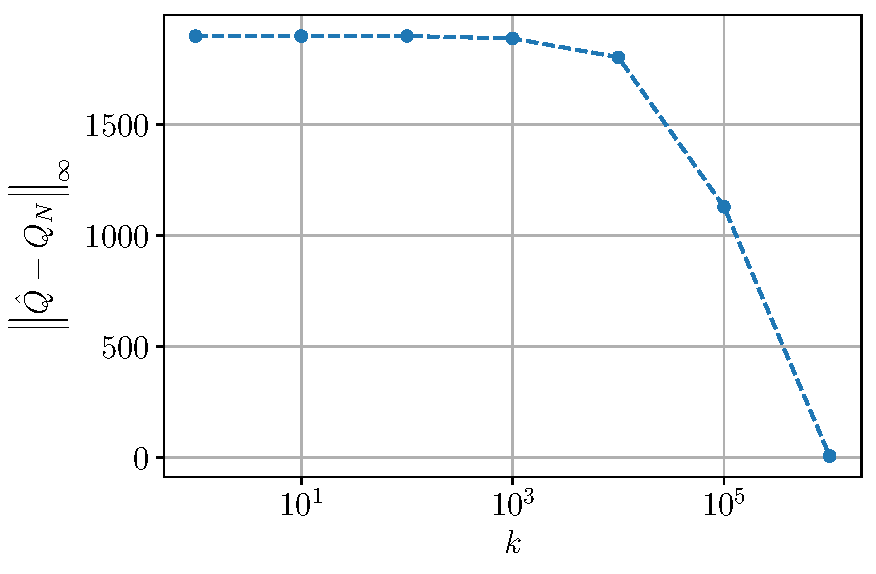
\includegraphics[width=\textwidth]{resources/pdf/5.1_deterministic.pdf}
            \caption{Deterministic domain.}
        \end{subfigure}
        \hfill
        \begin{subfigure}[b]{0.47\textwidth}
            \centering
            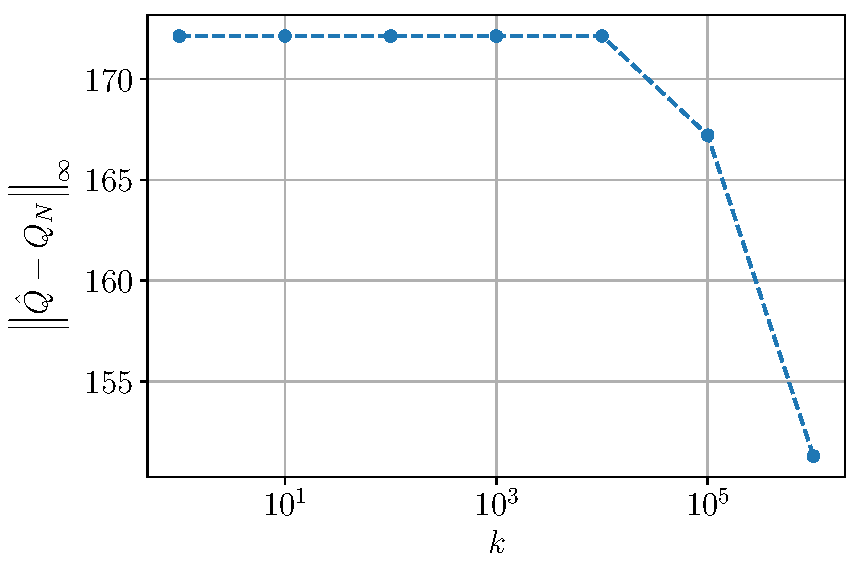
\includegraphics[width=\textwidth]{resources/pdf/5.1_stochastic.pdf}
            \caption{Stochastic domain.}
        \end{subfigure}
        \caption{Convergence of $\hat{Q}$ towards $Q_N$; $N = 1966$.}
        \label{fig:ql.convergence.speeds}
    \end{figure}
    
    One can see that the chosen time horizon $T = \num{e6}$ is (just) sufficient to have convergence of $\hat{Q}$ towards $Q_N$ in the deterministic domain. Conversely, it seems convergence was not reached in the stochastic domain as the infinite norm barely decreased. As before, for the sake of simplicity, we kept the last of $\hat{Q}$ for the rest of our calculations.
    
    An approximated optimal policy $\hat{\mu}^*$ can be directly derived from $\hat{Q}$ by replacing $Q_N$ by $\hat{Q}$ in relation \eqref{eq:N-optimal.policy}. The obtained policies, for both domains, are shown in Tables \ref{tab:ql.mu.star.deterministic} et \ref{tab:ql.mu.star.stochastic}.
    
    \begin{table}[h]
        \centering
        \begin{tabular}{c|c|c|c|c|c}
            \diagbox{$x$}{$y$} & $\bm{0}$ & $\bm{1}$ & $\bm{2}$ & $\bm{3}$ & $\bm{4}$ \\ \hline
            $\bm{0}$ & (1, 0) & (0, 1) & (0, 1) & (0, 1) & (-1, 0) \\ \hline
            $\bm{1}$ & (0, 1) & (0, 1) & (0, 1) & (0, 1) & (-1, 0) \\ \hline
            $\bm{2}$ & (-1, 0) & (0, 1) & (-1, 0) & (-1, 0) & (-1, 0) \\ \hline
            $\bm{3}$ & (-1, 0) & (0, 1) & (0, 1) & (-1, 0) & (-1, 0) \\ \hline
            $\bm{4}$ & (-1, 0) & (0, 1) & (-1, 0) & (-1, 0) & (0, -1) \\
        \end{tabular}
        \caption{$\hat{\mu}^*(x, y)$ for all $(x, y) \in X$ in the deterministic domain.}
        \label{tab:ql.mu.star.deterministic}
    \end{table}
    
    \begin{table}[h]
        \centering
        \begin{tabular}{c|c|c|c|c|c}
            \diagbox{$x$}{$y$} & $\bm{0}$ & $\bm{1}$ & $\bm{2}$ & $\bm{3}$ & $\bm{4}$ \\ \hline
            $\bm{0}$ & (1, 0) & (1, 0) & (1, 0) & (1, 0) & (-1, 0) \\ \hline
            $\bm{1}$ & (1, 0) & (0, -1) & (0, 1) & (0, -1) & (-1, 0) \\ \hline
            $\bm{2}$ & (-1, 0) & (0, -1) & (-1, 0) & (-1, 0) & (-1, 0) \\ \hline
            $\bm{3}$ & (-1, 0) & (0, -1) & (-1, 0) & (0, -1) & (0, -1) \\ \hline
            $\bm{4}$ & (-1, 0) & (-1, 0) & (-1, 0) & (0, 1) & (1, 0) \\
        \end{tabular}
        \caption{$\hat{\mu}^*(x, y)$ for all $(x, y) \in X$ in the stochastic domain.}
        \label{tab:ql.mu.star.stochastic}
    \end{table}
    
    Using the routine inspired from \eqref{eq:j.formulae}, we get $J^{\mu^*_N}_N$ (\cf{} Tables \ref{tab:j.optimal.values.deterministic} and \ref{tab:j.optimal.values.stochastic}), previously computed, along with $J^{\hat{\mu}^*}_N$ (\cf{} Tables \ref{tab:ql.j.deterministic} and \ref{tab:ql.j.stochastic}) for each state $(x, y)$ in both domains.
    
    \begin{table}[h]
        \centering
        \begin{tabular}{c|c|c|c|c|c}
            \diagbox{$x$}{$y$} & $\bm{0}$ & $\bm{1}$ & $\bm{2}$ & $\bm{3}$ & $\bm{4}$ \\ \hline
            $\bm{0}$ & \num{1842.031} & \num{1857.19} & \num{1881} & \num{1900} & \num{1900} \\ \hline
            $\bm{1}$ & \num{1854.576} & \num{1870.279} & \num{1880.09} & \num{1891} & \num{1900} \\ \hline
            $\bm{2}$ & \num{1842.031} & \num{1855.576} & \num{1870.279} & \num{1881.09} & \num{1891} \\ \hline
            $\bm{3}$ & \num{1828.61} & \num{1848.01} & \num{1863.646} & \num{1863.279} & \num{1864.09} \\ \hline
            $\bm{4}$ & \num{1816.324} & \num{1826.52} & \num{1849.01} & \num{1863.646} & \num{1842.01} \\
        \end{tabular}
        \caption{$J^{\hat{\mu}^*}_N(x, y)$ for all $(x, y) \in X$ in the deterministic domain; $N = 1966$.}
        \label{tab:ql.j.deterministic}
    \end{table}
    
    \begin{table}[h]
        \centering
        \begin{tabular}{c|c|c|c|c|c}
            \diagbox{$x$}{$y$} & $\bm{0}$ & $\bm{1}$ & $\bm{2}$ & $\bm{3}$ & $\bm{4}$ \\ \hline
            $\bm{0}$ & \num{133.445} & \num{132.11} & \num{136.081} & \num{136.415} & \num{146.644} \\ \hline
            $\bm{1}$ & \num{133.11} & \num{133.445} & \num{136.415} & \num{136.081} & \num{146.644} \\ \hline
            $\bm{2}$ & \num{133.445} & \num{133.11} & \num{136.081} & \num{136.415} & \num{142.144} \\ \hline
            $\bm{3}$ & \num{133.11} & \num{133.445} & \num{133.915} & \num{132.843} & \num{139.813} \\ \hline
            $\bm{4}$ & \num{133.445} & \num{126.11} & \num{132.843} & \num{136.743} & \num{136.743} \\
        \end{tabular}
        \caption{$J^{\hat{\mu}^*}_N(x, y)$ for all $(x, y) \in X$ in the stochastic domain; $N = 1966$.}
        \label{tab:ql.j.stochastic}
    \end{table}
    
    Once again, due to the convergence issue, one can see that values of $J^{\mu^*_N}_N$ and $J^{\hat{\mu}^*_N}_N$ are the same in the deterministic domain while they are different in the stochastic case.
    
    \subsection{Online Q-learning}\label{sec:online.q.learning}
    
    For this section, the trajectory has to be generated according to an $\epsilon$-greedy policy, \ie{} an exploratory policy that selects with a probability $\epsilon$ a random action and a probability $1 - \epsilon$ the action recommended by the approximated policy $\hat{\mu}^*$.
    \begin{equation}\label{eq:epsilon-greedy}
        \begin{cases}
            u_k \sim \mathcal{U}\{U\} & \text{with probability } \epsilon \\
            u_k = \hat{\mu}^*(x_k) & \text{else} \\
        \end{cases}
    \end{equation}
    Because this policy uses $\hat{\mu}^*$, it requires to know the \emph{current} values of $\hat{Q}$. Therefore, we have to implement an online Q-learning protocol. In order to keep the code simple, we implemented this protocol as a function with a few parameters such that the three requested experiments were easy to setup and repeat.
    
    It was also requested to measure the performance of the agent(s) with the metric $\norm{\hat{Q} - J^{\mu^*_N}_N}_\infty$ after each episode. However, $Q$ and $J^\mu_N$ don't have the same domain and therefore shouldn't be compared directly with the infinite norm. To allow this comparison, we decided to \emph{project} $\hat{Q}$ with respect to $\hat{\mu}^*$, \ie{}
    \begin{equation}
        \norm{\hat{Q} - J^{\mu^*_N}_N}_\infty = \sup_{x \in X} \abs{\hat{Q}(x, \hat{\mu}^*(x)) - J^{\mu^*_N}_N(x)} .
    \end{equation}
    
    \begin{figure}[h]
        \begin{subfigure}[b]{0.47\textwidth}
            \centering
            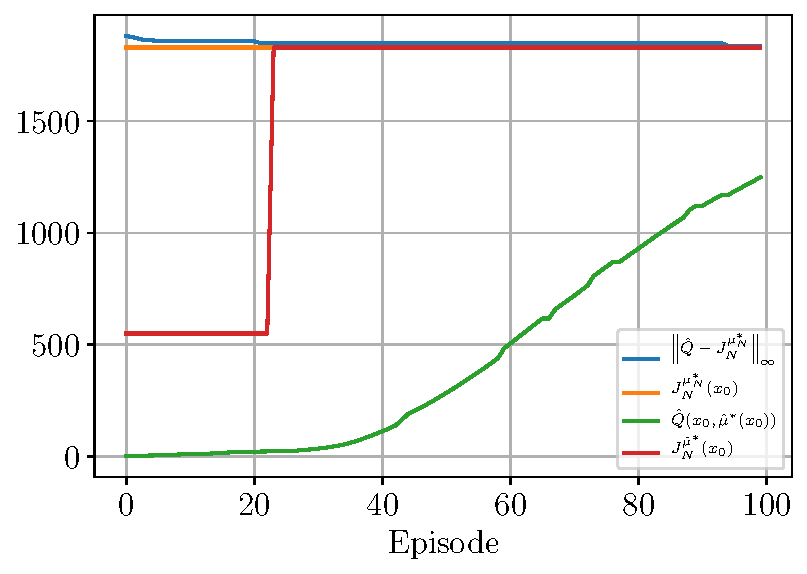
\includegraphics[width=\textwidth]{resources/pdf/5.2.1_deterministic.pdf}
            \caption{Deterministic domain.}
        \end{subfigure}
        \hfill
        \begin{subfigure}[b]{0.47\textwidth}
            \centering
            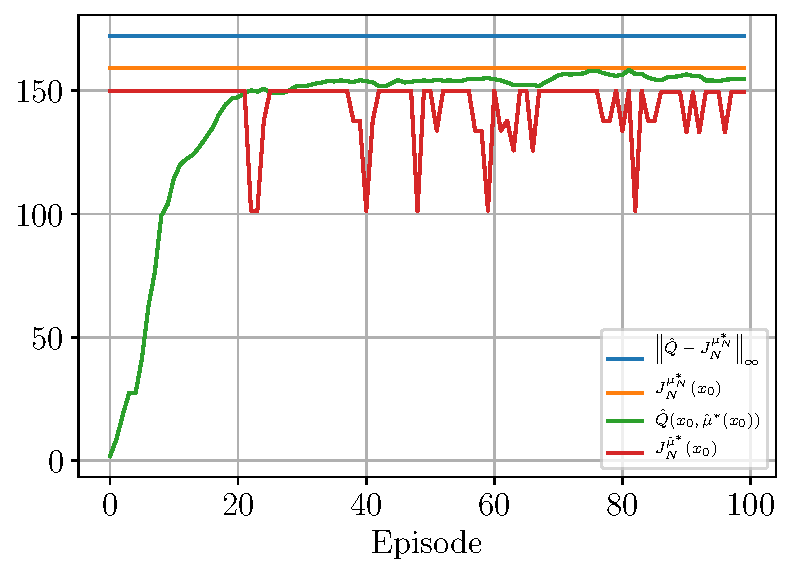
\includegraphics[width=\textwidth]{resources/pdf/5.2.1_stochastic.pdf}
            \caption{Stochastic domain.}
        \end{subfigure}
        \caption{Performance of the agent for the first experimental protocol.}
        \label{fig:ql.first.protocol}
    \end{figure}
    
    \begin{figure}[h]
        \begin{subfigure}[b]{0.47\textwidth}
            \centering
            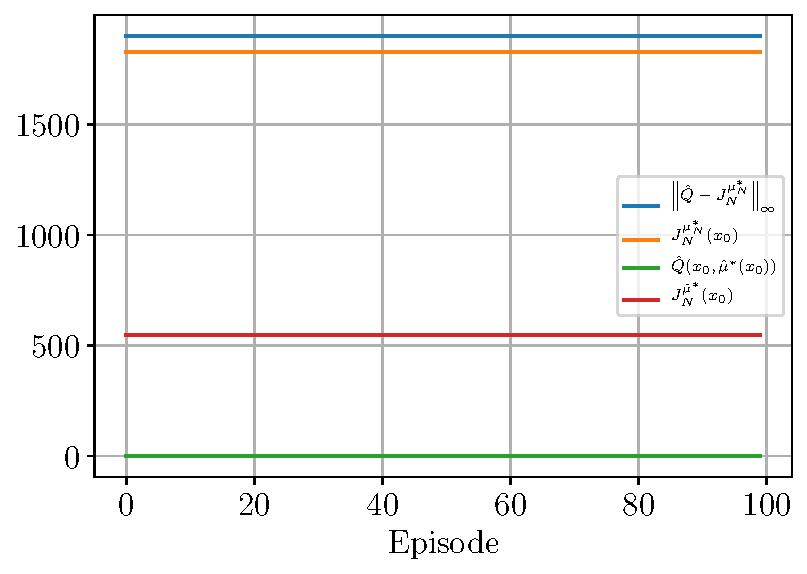
\includegraphics[width=\textwidth]{resources/pdf/5.2.2_deterministic.pdf}
            \caption{Deterministic domain.}
        \end{subfigure}
        \hfill
        \begin{subfigure}[b]{0.47\textwidth}
            \centering
            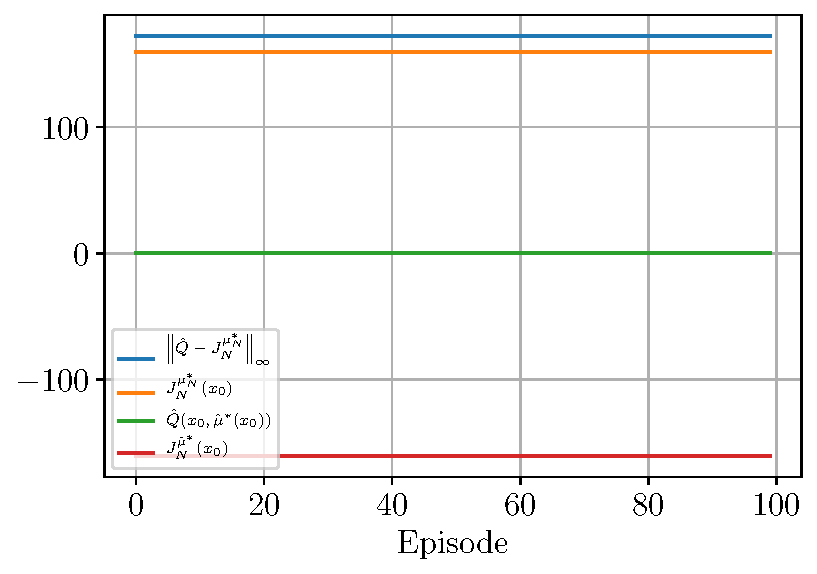
\includegraphics[width=\textwidth]{resources/pdf/5.2.2_stochastic.pdf}
            \caption{Stochastic domain.}
        \end{subfigure}
        \caption{Performance of the agent for the first experimental protocol.}
        \label{fig:ql.second.protocol}
    \end{figure}
    
    \begin{figure}[h]
        \begin{subfigure}[b]{0.47\textwidth}
            \centering
            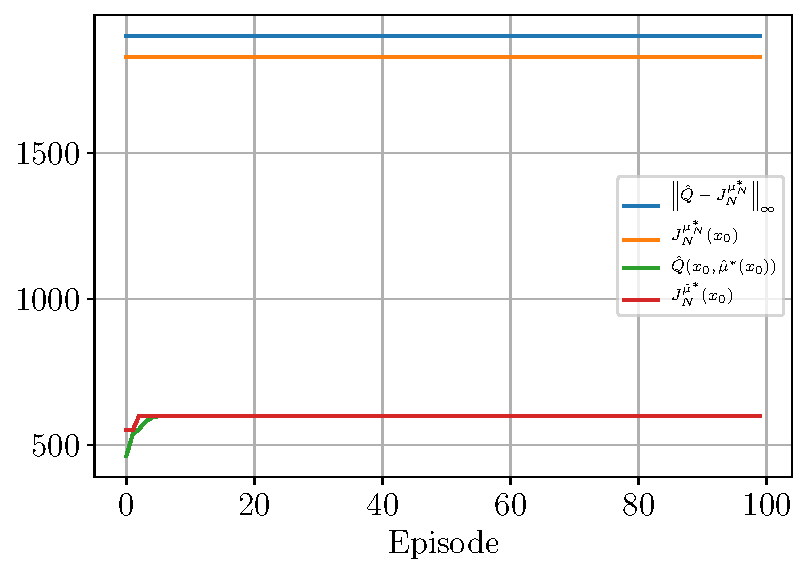
\includegraphics[width=\textwidth]{resources/pdf/5.2.3_deterministic.pdf}
            \caption{Deterministic domain.}
        \end{subfigure}
        \hfill
        \begin{subfigure}[b]{0.47\textwidth}
            \centering
            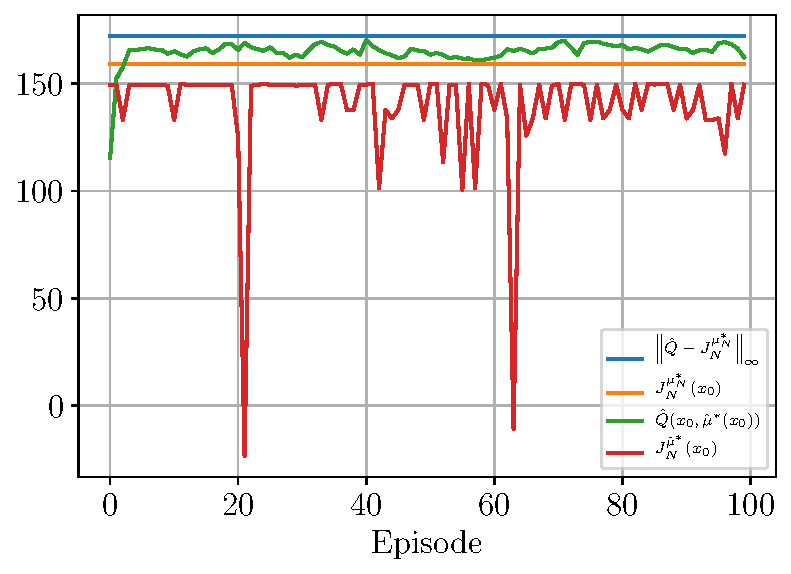
\includegraphics[width=\textwidth]{resources/pdf/5.2.3_stochastic.pdf}
            \caption{Stochastic domain.}
        \end{subfigure}
        \caption{Performance of the agent for the first experimental protocol.}
        \label{fig:ql.third.protocol}
    \end{figure}
    
    Unfortunately, as can be seen in Figures \ref{fig:ql.first.protocol}, \ref{fig:ql.second.protocol} and \ref{fig:ql.third.protocol}, this metric doesn't seem to converge towards zero as the agent learns. In fact, this metric isn't well suited to measure the performance of the agent(s).
    
    Indeed, a drawback of the $\epsilon$-greedy policy is that it will much more rarely explore state-action pairs $(x, u)$ leading to low rewards than a random uniform policy. As a consequence, the value of $\hat{Q}(x, u)$ for such pair is very far from $J^{\mu^*_N}_N(x)$ since the algorithm \ref{meth:q.learning.algorithm} requires a large (infinite) number of visits to be accurate.
    
    However, the $\epsilon$-greedy policy has the advantage to explore quite well the \enquote{good} trajectories. Therefore, as the initial state is $x_0 = (3, 0)$, it should determine accurately the expected return of this state and the optimal policy starting from it. These two quantities are respectively measured as $\hat{Q}(x_0, \hat{\mu}^*(x_0))$ and $J^{\hat{\mu}^*}_N(x_0)$ and should ideally both converge towards $J^{\mu^*_N}_N(x_0)$.
    
    As can be seen in Figure \ref{fig:ql.first.protocol}, these two quantities do seem to converge in the first experiment although less consistently in the stochastic domain. For the second experiment, however, no convergence can be observed whatsoever. This can be easily explained as $\alpha_k$ decreases exponentially\footnotemark{} quickly with $k$. Indeed, by $k = 100$, \ie{} a tenth of the first episode, $\alpha_k \simeq \num{e-11}$ which is numerically insignificant. Hence, $\hat{Q}$ is only modified on the first few updates.
    
    \footnotetext{In fact, $\alpha_k = 0.8^k \alpha_0$ isn't a valid strategy as it is required that $\sum^T_{k = 0} \alpha_k$ diverges to $\infty$ as $T$ grows.}
    
    For the third experiment (\cf{} Figure \ref{fig:ql.third.protocol}), the metrics seem to reach a plateau after a few episodes. It could be explained by the fact that, in the buffer, which is simply the past trajectory, a lot of sub-optimal transitions are represented since they were chosen (partly) using a sub-optimal $\hat{Q}$. Therefore, sampling from this buffer further anchors those transitions in $\hat{Q}$ and a lock is reached. Theoretically, this lock should eventually resolve as the values of $\hat{Q}$ cannot grow past $\frac{B_r}{1 - \gamma}$.
    
    A way to resolve the lock faster, is to increase the stochasticity of the transitions. For example, one could increase $\epsilon$ to $0.5$, reduce the number of transitions sampled from the buffer, limit the size of the buffer, clear the buffer after each episode, etc. We tried some of these in our implementation but didn't have the time to analyze them.
    
    \subsection{Discount factor}
    
    As requested, we have re-run the first experimental protocol of Section \ref{sec:online.q.learning} with $\gamma = \num{0.4}$ (\cf{} Figure \ref{fig:ql.first.protocol.gamma}).
    
    \begin{figure}[h]
        \begin{subfigure}[b]{0.47\textwidth}
            \centering
            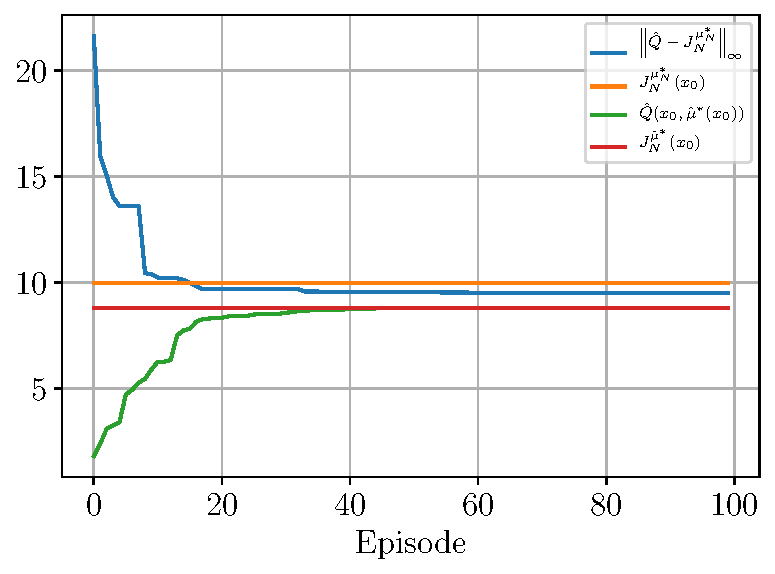
\includegraphics[width=\textwidth]{resources/pdf/5.3_deterministic.pdf}
            \caption{Deterministic domain.}
        \end{subfigure}
        \hfill
        \begin{subfigure}[b]{0.47\textwidth}
            \centering
            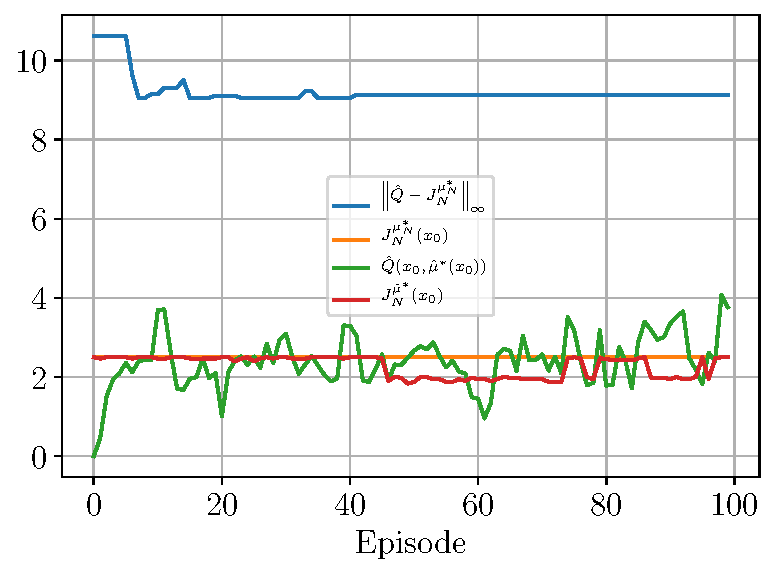
\includegraphics[width=\textwidth]{resources/pdf/5.3_stochastic.pdf}
            \caption{Stochastic domain.}
        \end{subfigure}
        \caption{Performance of the agent for the first experimental protocol; $\gamma = \num{0.4}$.}
        \label{fig:ql.first.protocol.gamma}
    \end{figure}
    
    It seems like the metrics converge faster towards their goal. It might be explained by the fact that the goal is lower and can be attained in shorter trajectories as $\gamma$ is much lower.
    
    \subsection{Q-learning with Another Exploration Policy}
    
    We choose, as an other exploration policy, the \emph{Boltzmann exploration policy}. In this policy, the probability of selecting an action $u$ in a state $x$ is given by
    
    \begin{equation}
        \frac{\tau \exp \hat{Q}(x, u)}{\tau \sum_{u' \in U} \exp \hat{Q}(x, u')} .
    \end{equation}
    
    In our implementation we chose $\tau = \frac{1 - \gamma}{B_r}$ as it is (the inverse of) a bound for the values of $Q$. This prevents to have completely skewed distributions. This policy is more stochastic that the $\epsilon$-greedy one, and therefore should converge more consistently.
    
    We have re-run the first experimental protocol of Section \ref{sec:online.q.learning} with this new exploration policy (\cf{} Figure \ref{fig:ql.first.protocol.boltzmann}).
    
    \begin{figure}[h]
        \begin{subfigure}[b]{0.47\textwidth}
            \centering
            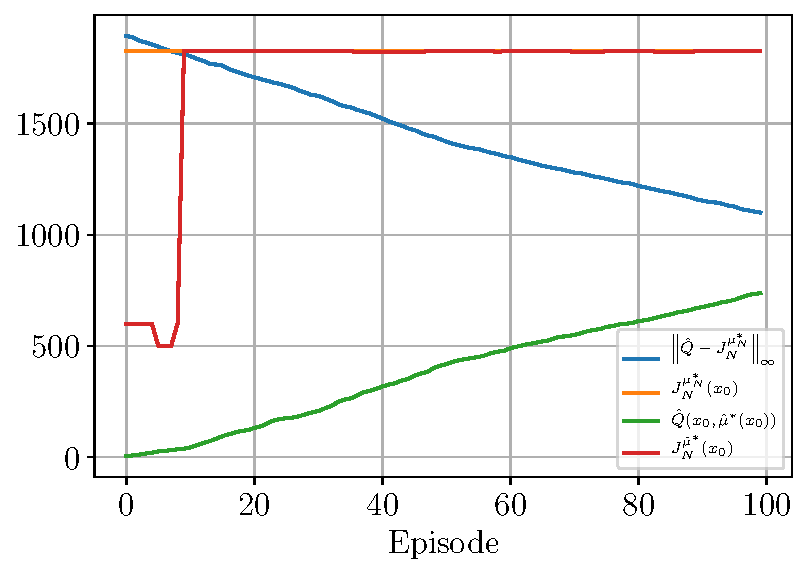
\includegraphics[width=\textwidth]{resources/pdf/5.4_deterministic.pdf}
            \caption{Deterministic domain.}
        \end{subfigure}
        \hfill
        \begin{subfigure}[b]{0.47\textwidth}
            \centering
            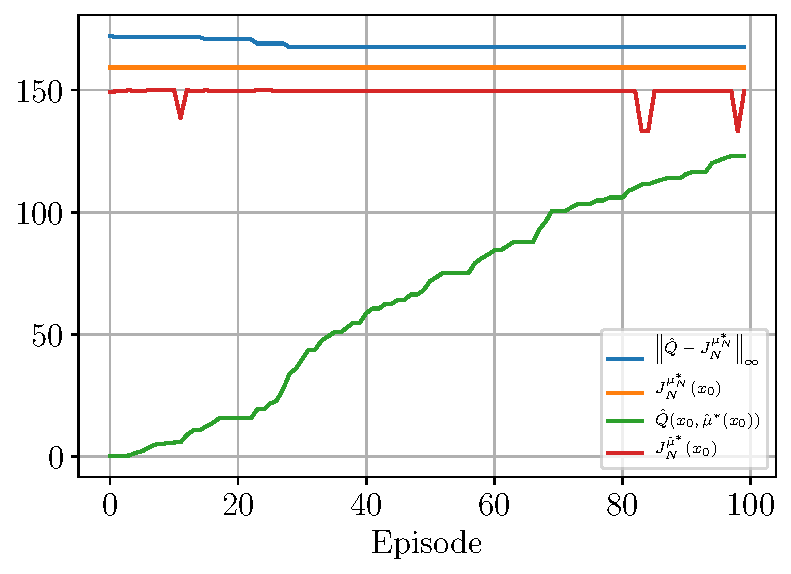
\includegraphics[width=\textwidth]{resources/pdf/5.4_stochastic.pdf}
            \caption{Stochastic domain.}
        \end{subfigure}
        \caption{Convergence speeds of $\hat{Q}$ towards $J^{\mu^*}_N$ for the first experimental protocol; Boltzmann exploration policy.}
        \label{fig:ql.first.protocol.boltzmann}
    \end{figure}
    
    As expected, the metrics converge very consistently in both domains, although not as fast as with $\epsilon$-greedy. This is not very surprising as, in our setting, this policy is very similar to a random uniform policy.

    \newpage

    \printbibliography
\end{document}
